\documentclass{article}
\usepackage[utf8]{inputenc}
\usepackage{mathtools}
\usepackage{graphicx}
\usepackage{hyperref}

\setlength{\parindent}{0pt}

\title{AerE 161 \\ Project \#2: Flight Path of a Projectile}
\author{Hammad Imam \\ Undergraduate, Aerospace Engineering \\ Iowa State University}
\date{March 23rd,	2018}

\begin{document}

\begin{titlepage}
\maketitle
\end{titlepage}

\clearpage
\tableofcontents

\newpage

\section{Problem Statement}
The purpose of this assignment was to study the effects of air resistance on the flight path of projectiles. Since objects behave differently with and without air resistance, two formulas were used to calculate trajectories. This project utilizes 5 different .m files to calculate the data, plot different graphs, and to pass values to be calculated and plotted. As the output, 6 graphs were generated.

\newpage
\section{Theory}
\subsection{Introduction}
In this section, the methods of calculation for 

\newpage
\section{Solution}
\subsection{Overview}
\subsection{Code}
\subsubsection{flightpath.m}
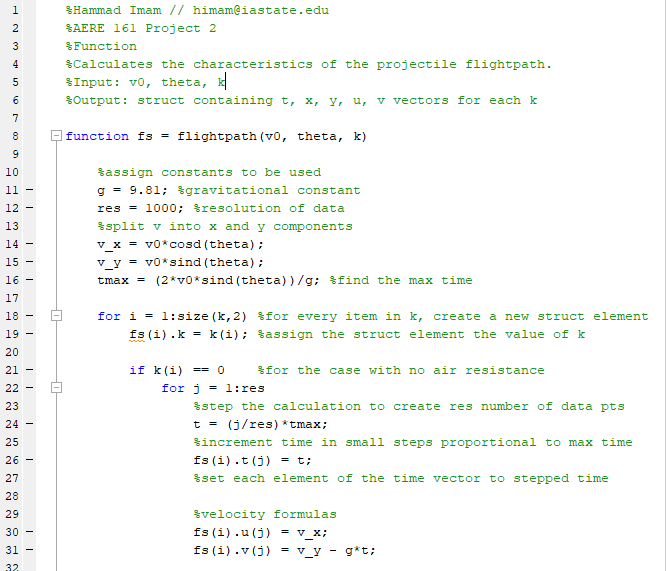
\includegraphics [width=\linewidth]{code_flightpath1.png}
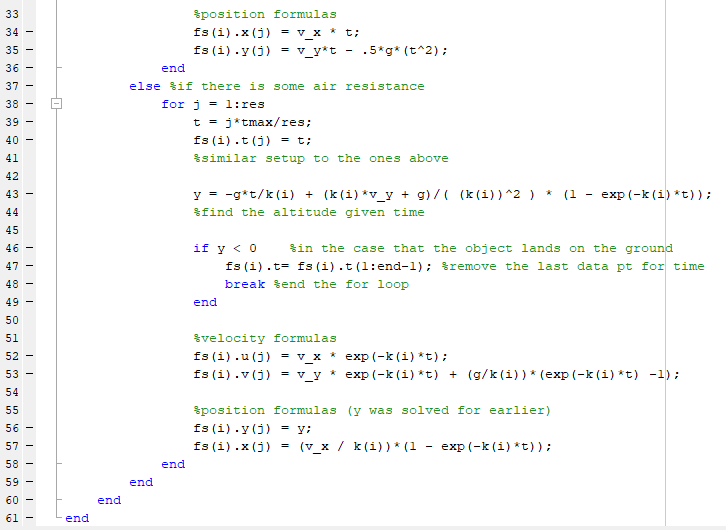
\includegraphics [width=\linewidth]{code_flightpath2.png}
\subsubsection{plot_flightpaths.m}
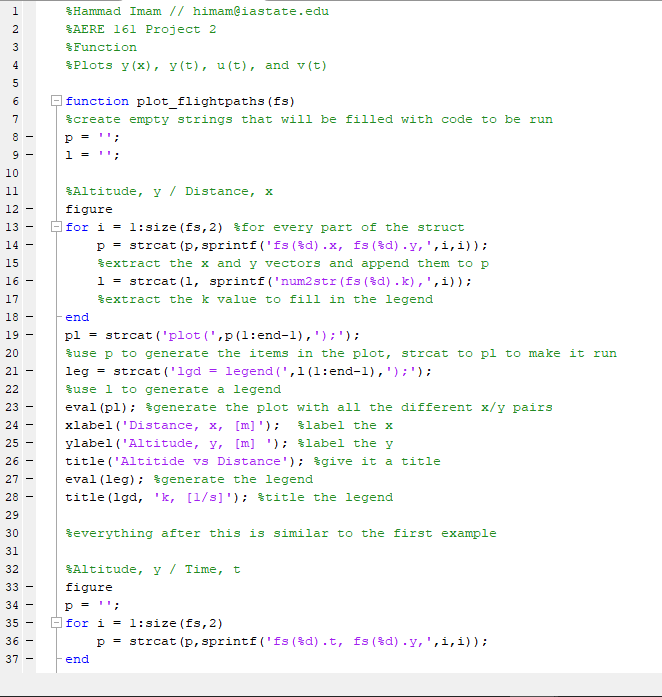
\includegraphics [width=\linewidth]{code_plot_flightpaths1.png}
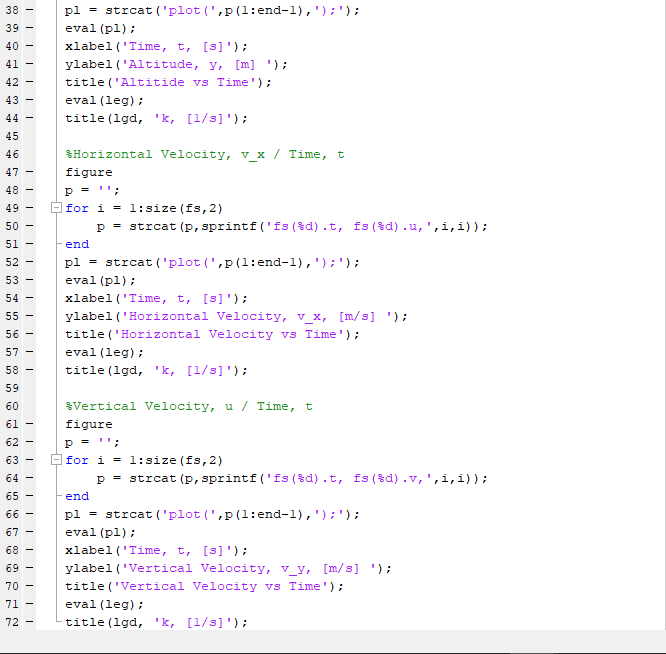
\includegraphics [width=\linewidth]{code_plot_flightpaths2.png}
\subsubsection{main_flightpaths.m}
\includegraphics [width=\linewidth]{code_main_flightpaths1.png}
\subsubsection{plot_range.m}
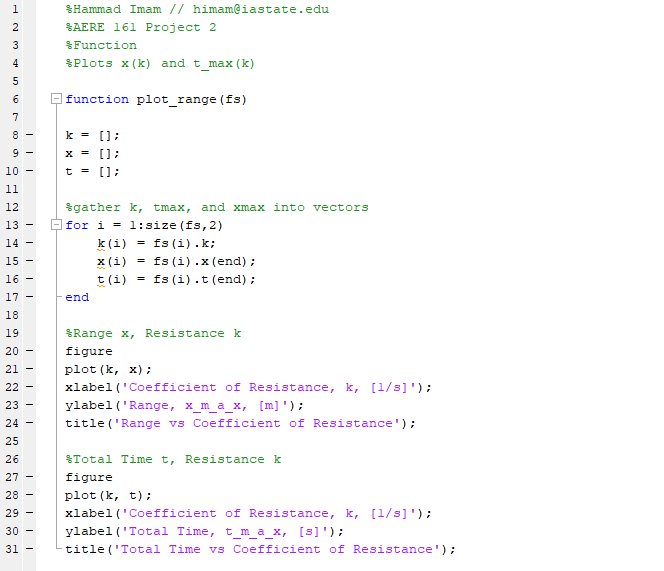
\includegraphics [width=\linewidth]{code_plot_range.png}
\subsubsection{main_range.m}
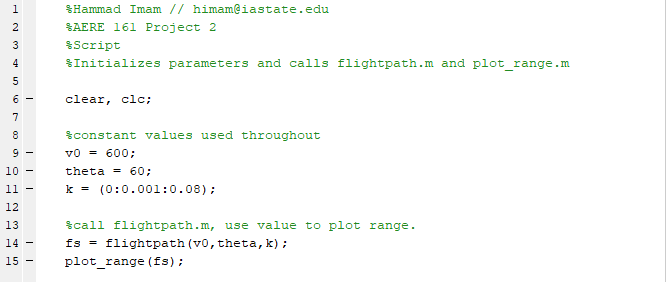
\includegraphics [width=\linewidth]{code_main_range.png}
\subsection{Plots}
\subsection{}


\newpage
\section{Discussion}
\subsection{Analysis}
\subsection{Challenges}

\end{document}
